\documentclass[11pt,a4paper]{article}
\usepackage[utf8]{inputenc}
\usepackage{amsmath,amssymb,amsthm}
\usepackage{graphicx}
\usepackage{tikz}
\usepackage{pgfplots}
\usepackage{algorithm}
\usepackage{algorithmic}
\usepackage{hyperref}
\usepackage{geometry}
\usepackage{booktabs}
\usepackage{multirow}

\geometry{margin=1in}
\pgfplotsset{compat=1.17}
\usetikzlibrary{arrows.meta,positioning,shapes.geometric,calc}

\newtheorem{theorem}{Theorem}
\newtheorem{lemma}{Lemma}
\newtheorem{definition}{Definition}
\newtheorem{proposition}{Proposition}

\title{\textbf{NeuroGen V1: Evolutionary and Local-Learning Based Neural Networks Without Backpropagation}}

\author{
Viraaj Sharma\\
AI Researcher, Anomaly Labs\\
\texttt{viraaj@anomalylabs.ai}
\and
Satnam Singh\\
AI Researcher, Anomaly Labs\\
\texttt{satnam@anomalylabs.ai}
}

\date{\today}

\begin{document}

\maketitle

\begin{abstract}
Backpropagation has dominated neural network training for decades, yet it suffers from biological implausibility, credit assignment challenges, and computational constraints in distributed systems. We present \textbf{NeuroGen V1}, a novel framework combining evolutionary algorithms with local Hebbian-style plasticity rules to train neural networks without gradient descent. Our approach encodes network topologies as evolvable genomes, applies neuroevolutionary operators for structural search, and employs local learning rules (Hebbian, Oja's rule, BCM theory) for synaptic weight adaptation during lifetime. We formalize this as a bilevel optimization problem where evolution optimizes architecture and plasticity parameters while local rules optimize weights. Through rigorous mathematical analysis, we prove convergence properties and derive computational complexity bounds. Experimental validation on XOR, noisy XOR, and 3-bit parity problems demonstrates competitive performance with evolved networks achieving 95-100\% accuracy. Ablation studies reveal critical insights into population dynamics, mutation strategies, and plasticity mechanisms. This work establishes a foundation for biologically-inspired, backprop-free learning systems with applications in neuromorphic computing and distributed AI.
\end{abstract}

\noindent\textbf{Keywords:} Neuroevolution, Local Learning Rules, Hebbian Plasticity, Evolutionary Algorithms, Backpropagation-Free Learning, Neuromorphic Computing

\section{Introduction}

\subsection{Motivation and Background}

Backpropagation \cite{rumelhart1986learning}, while computationally efficient, presents fundamental limitations that motivate alternative learning paradigms. First, the \textit{biological implausibility} of error signal propagation through symmetric weights contradicts neuroscientific evidence \cite{crick1989recent}. Second, backpropagation requires \textit{global coordination} and differentiability, making it unsuitable for distributed, asynchronous systems. Third, the algorithm struggles with \textit{credit assignment} in deep networks and recurrent architectures \cite{bengio2015towards}.

Nature, by contrast, employs two complementary mechanisms: \textbf{evolution} operates on phylogenetic timescales to optimize network structure and learning rules, while \textbf{local plasticity} enables rapid adaptation during an organism's lifetime through synapse-specific modifications \cite{hebb1949organization}. This duality inspires our framework.

\subsection{Evolutionary and Plastic Learning}

\textbf{Neuroevolution} searches the space of network architectures and parameters using evolutionary algorithms. Methods like NEAT \cite{stanley2002evolving}, HyperNEAT \cite{stanley2009hypercube}, and Evolution Strategies \cite{salimans2017evolution} have shown promise but often evolve static networks. \textbf{Local learning rules}—including Hebbian learning \cite{hebb1949organization}, Oja's rule \cite{oja1982simplified}, and BCM theory \cite{bienenstock1982theory}—provide biologically plausible weight update mechanisms based solely on pre- and post-synaptic activity.

The key insight of NeuroGen V1 is to \textit{evolve networks capable of learning}, combining structural search with adaptive plasticity. Evolution discovers architectures and plasticity hyperparameters, while local rules refine weights during evaluation.

\subsection{Contributions}

Our main contributions are:

\begin{itemize}
\item \textbf{Formal Framework:} Mathematical formalization of genome encoding, mutation operators, and forward propagation with rigorous acyclicity guarantees (Theorem \ref{thm:acyclic}).
\item \textbf{Bilevel Optimization:} Formulation of evolution + plasticity as a bilevel problem with convergence analysis (Theorem \ref{thm:convergence}).
\item \textbf{Local Learning Derivations:} Detailed mathematical derivations of Hebbian, Oja, and BCM rules with stability proofs (Lemmas \ref{lem:hebbian_stability}--\ref{lem:bcm_stability}).
\item \textbf{Computational Complexity:} Tight bounds on forward pass, mutation, and evolution complexity (Theorem \ref{thm:complexity}).
\item \textbf{Empirical Validation:} Experiments on XOR, noisy XOR, and 3-bit parity with comprehensive ablation studies.
\item \textbf{Extensive Appendices:} Pseudocode, proofs, additional experiments, genome examples, hyperparameters, and TikZ diagrams.
\end{itemize}

\section{Background and Related Work}

\subsection{Neuroevolution}

\textbf{NEAT} (NeuroEvolution of Augmenting Topologies) \cite{stanley2002evolving} pioneered topology evolution through incremental complexification, speciation, and innovation tracking. \textbf{HyperNEAT} extended this with compositional pattern-producing networks (CPPNs) for geometric encodings. \textbf{Evolution Strategies} \cite{salimans2017evolution} demonstrated scalability on RL tasks by evolving weight perturbations. However, these methods typically evolve \textit{fixed} networks without lifetime learning.

\subsection{Local Learning Rules}

\textbf{Hebbian Learning} \cite{hebb1949organization} posits "cells that fire together, wire together," formalized as:
\begin{equation}
\Delta w_{ij} = \eta \, x_i \, y_j
\end{equation}
where $x_i$ is pre-synaptic activity, $y_j$ is post-synaptic activity, and $\eta$ is the learning rate. This rule is unstable without normalization.

\textbf{Oja's Rule} \cite{oja1982simplified} adds weight decay for stability:
\begin{equation}
\Delta w_{ij} = \eta \, y_j \left( x_i - y_j w_{ij} \right)
\end{equation}

\textbf{BCM Theory} \cite{bienenstock1982theory} introduces a sliding threshold $\theta$ for selectivity:
\begin{equation}
\Delta w_{ij} = \eta \, x_i \, y_j \left( y_j - \theta \right)
\end{equation}

\subsection{Backpropagation Alternatives}

Recent work explores alternatives including feedback alignment \cite{lillicrap2016random}, target propagation \cite{lee2015difference}, and predictive coding \cite{whittington2017approximation}. Evolutionary meta-learning \cite{schmidhuber1987evolutionary} evolves learning rules themselves. Our work combines structural evolution with fixed local rules.

\subsection{Neuromorphic Relevance}

Neuromorphic hardware \cite{davies2018loihi} emphasizes local computation and asynchronous updates, aligning naturally with our framework. Spike-timing-dependent plasticity (STDP) \cite{markram1997regulation} shares conceptual similarities with our local rules.

\section{Methods}

\subsection{Genome Formalization}

\begin{definition}[Genome]
A genome $G = (V, E, \Theta)$ consists of:
\begin{itemize}
\item $V = \{v_1, \ldots, v_n\}$: set of nodes (neurons)
\item $E \subseteq V \times V$: set of directed edges (synapses)
\item $\Theta$: parameter set including weights $w_{ij}$, biases $b_i$, activation functions $\sigma_i$, and plasticity hyperparameters $\{\eta_i, \theta_i\}$
\end{itemize}
\end{definition}

Each node $v_i$ has:
\begin{itemize}
\item Type: $\tau_i \in \{\text{input}, \text{hidden}, \text{output}\}$
\item Activation: $\sigma_i \in \{\text{tanh}, \text{sigmoid}, \text{relu}, \text{linear}\}$
\item Bias: $b_i \in \mathbb{R}$
\item Plasticity rate: $\eta_i \in [0, 1]$
\item Threshold (BCM): $\theta_i \in \mathbb{R}^+$
\end{itemize}

Each edge $(v_i, v_j) \in E$ has:
\begin{itemize}
\item Weight: $w_{ij} \in [-w_{\max}, w_{\max}]$
\item Innovation number: $\text{innov}_{ij} \in \mathbb{N}$ (for crossover alignment)
\item Plasticity rule: $\rho_{ij} \in \{\text{Hebbian}, \text{Oja}, \text{BCM}, \text{static}\}$
\end{itemize}

\subsection{Acyclic Graph Constraint}

\begin{theorem}[Acyclicity]\label{thm:acyclic}
Let $G = (V, E, \Theta)$ be a genome. Define a topological ordering $\prec$ on $V$ such that for all $(v_i, v_j) \in E$, we have $v_i \prec v_j$. Then $G$ is acyclic if and only if such an ordering exists.
\end{theorem}

\begin{proof}
($\Rightarrow$) Assume $G$ is acyclic. Perform depth-first search (DFS) from input nodes, assigning levels $\ell(v_i)$ as the maximum path length from any input. Define $v_i \prec v_j \iff \ell(v_i) < \ell(v_j)$. Since $G$ is acyclic, no back edges exist, so this ordering is well-defined.

($\Leftarrow$) Assume ordering $\prec$ exists. Suppose for contradiction that a cycle $v_{i_1} \to v_{i_2} \to \cdots \to v_{i_k} \to v_{i_1}$ exists. Then $v_{i_1} \prec v_{i_2} \prec \cdots \prec v_{i_k} \prec v_{i_1}$, implying $v_{i_1} \prec v_{i_1}$, contradicting irreflexivity of $\prec$.
\end{proof}

We maintain acyclicity by assigning each node a \textit{layer index} $\ell(v_i)$ and only allowing edges $(v_i, v_j)$ where $\ell(v_i) < \ell(v_j)$.

\subsection{Mutation Operators}

\subsubsection{Add Node Mutation}

Select edge $(v_i, v_j) \in E$ with probability $p_{\text{add\_node}}$. Disable $(v_i, v_j)$ and insert new node $v_k$ with edges $(v_i, v_k)$ and $(v_k, v_j)$. Set $\ell(v_k) = \frac{\ell(v_i) + \ell(v_j)}{2}$ to preserve ordering. Initialize:
\begin{align}
w_{ik} &= w_{ij}, \quad w_{kj} = 1.0 \\
b_k &\sim \mathcal{N}(0, 0.1), \quad \sigma_k \sim \text{Uniform}(\{\text{tanh}, \text{sigmoid}, \text{relu}\})
\end{align}

\subsubsection{Add Connection Mutation}

Select nodes $v_i, v_j$ with $\ell(v_i) < \ell(v_j)$ and $(v_i, v_j) \notin E$ with probability $p_{\text{add\_conn}}$. Add edge with:
\begin{equation}
w_{ij} \sim \mathcal{N}(0, \sigma_w^2), \quad \rho_{ij} \sim \text{Uniform}(\{\text{Hebbian}, \text{Oja}, \text{BCM}, \text{static}\})
\end{equation}

\subsubsection{Weight Mutation}

For each $w_{ij}$, with probability $p_{\text{weight}}$:
\begin{equation}
w_{ij} \leftarrow \begin{cases}
\mathcal{N}(0, \sigma_w^2) & \text{with prob. } p_{\text{reset}} \\
w_{ij} + \mathcal{N}(0, \sigma_{\text{perturb}}^2) & \text{otherwise}
\end{cases}
\end{equation}
Clip to $[-w_{\max}, w_{\max}]$.

\subsubsection{Bias and Plasticity Mutation}

Mutate biases and plasticity hyperparameters similarly:
\begin{align}
b_i &\leftarrow b_i + \mathcal{N}(0, 0.05^2) \\
\eta_i &\leftarrow \text{clip}(\eta_i + \mathcal{N}(0, 0.01^2), 0, 1) \\
\theta_i &\leftarrow \max(0.01, \theta_i + \mathcal{N}(0, 0.05^2))
\end{align}

\subsection{Forward Propagation}

\begin{definition}[Forward Pass]
Given input $\mathbf{x} \in \mathbb{R}^{n_{\text{in}}}$, compute activations $a_i$ for all $v_i \in V$ in topological order:
\begin{equation}
a_i = \begin{cases}
x_i & \text{if } \tau_i = \text{input} \\
\sigma_i\left( \sum_{(v_j, v_i) \in E} w_{ji} a_j + b_i \right) & \text{otherwise}
\end{cases}
\end{equation}
Output is $\mathbf{y} = (a_i : \tau_i = \text{output})$.
\end{definition}

\subsection{Local Learning Rules}

\subsubsection{Hebbian Learning}

\begin{equation}
\Delta w_{ij} = \eta_i \, a_i \, a_j
\end{equation}

\begin{lemma}[Hebbian Instability]\label{lem:hebbian_stability}
Under Hebbian learning with constant input, weights grow unbounded: $\|w_{ij}(t)\| \to \infty$ as $t \to \infty$.
\end{lemma}

\begin{proof}
Let $a_i = c_i > 0$ constant. Then $w_{ij}(t+1) = w_{ij}(t) + \eta c_i c_j$, so $w_{ij}(t) = w_{ij}(0) + t \eta c_i c_j \to \infty$.
\end{proof}

\subsubsection{Oja's Rule}

\begin{equation}
\Delta w_{ij} = \eta_i \, a_j \left( a_i - a_j w_{ij} \right)
\end{equation}

\begin{lemma}[Oja Stability]\label{lem:oja_stability}
Under Oja's rule, weights converge to bounded values satisfying $\sum_j w_{ij}^2 \leq 1$.
\end{lemma}

\begin{proof}
Consider $\frac{d}{dt} \sum_j w_{ij}^2 = 2 \sum_j w_{ij} \Delta w_{ij} = 2\eta \sum_j w_{ij} a_j (a_i - a_j w_{ij})$. At equilibrium, $a_i = \sum_j a_j w_{ij}$, so:
\begin{equation}
\frac{d}{dt} \sum_j w_{ij}^2 = 2\eta a_i^2 - 2\eta \sum_j (a_j w_{ij})^2 \leq 0 \quad \text{when } \sum_j w_{ij}^2 \geq 1
\end{equation}
Thus weights remain bounded.
\end{proof}

\subsubsection{BCM Theory}

\begin{equation}
\Delta w_{ij} = \eta_i \, a_i \, a_j \left( a_j - \theta_i \right)
\end{equation}

Threshold updates:
\begin{equation}
\theta_i \leftarrow \alpha \theta_i + (1 - \alpha) a_j^2
\end{equation}

\begin{lemma}[BCM Selectivity]\label{lem:bcm_stability}
BCM learning drives weights to strengthen for high post-synaptic activity ($a_j > \theta_i$) and weaken for low activity ($a_j < \theta_i$), achieving selectivity.
\end{lemma}

\begin{proof}
When $a_j > \theta_i$, $\Delta w_{ij} > 0$ (potentiation). When $a_j < \theta_i$, $\Delta w_{ij} < 0$ (depression). The sliding threshold $\theta_i$ adapts to mean activity, ensuring selectivity.
\end{proof}

\subsection{Bilevel Optimization Formulation}

\begin{definition}[Bilevel Problem]
\begin{align}
\min_{G \in \mathcal{G}} \quad & F(G) = \mathbb{E}_{(\mathbf{x}, \mathbf{y}) \sim \mathcal{D}} \left[ \mathcal{L}(f_G(\mathbf{x}; w^*), \mathbf{y}) \right] \\
\text{s.t.} \quad & w^* = \arg\min_{w} \sum_{t=1}^T \mathcal{L}(f_G(\mathbf{x}_t; w_t), \mathbf{y}_t) \\
& w_{t+1} = w_t + \Delta w_t \quad (\text{local rule})
\end{align}
\end{definition}

Here, the \textit{upper level} (evolution) optimizes genome $G$ to minimize expected loss, while the \textit{lower level} (plasticity) optimizes weights $w$ via local rules during lifetime.

\begin{theorem}[Convergence]\label{thm:convergence}
Under bounded plasticity rates $\eta_i \in [0, \eta_{\max}]$ and Lipschitz loss $\mathcal{L}$, the bilevel optimization converges to a local optimum with probability 1 as population size $N \to \infty$ and generations $T \to \infty$.
\end{theorem}

\begin{proof}[Proof Sketch]
Evolution performs stochastic search over $\mathcal{G}$. By the law of large numbers, fitness estimates converge to true expected fitness. Selection pressure drives the population toward high-fitness regions. Local learning ensures weights adapt within each genome's lifetime, improving fitness estimates. Combining these, the population converges to a local optimum in the joint space of architectures and plasticity rules. Full proof in Appendix B.
\end{proof}

\subsection{Computational Complexity}

\begin{theorem}[Complexity Bounds]\label{thm:complexity}
Let $n = |V|$, $m = |E|$, $N$ = population size, $T$ = generations, $L$ = lifetime steps. Then:
\begin{itemize}
\item Forward pass: $O(m + n)$
\item Plasticity update: $O(m)$
\item Mutation: $O(n + m)$
\item Single generation: $O(N \cdot L \cdot m)$
\item Total evolution: $O(N \cdot T \cdot L \cdot m)$
\end{itemize}
\end{theorem}

\begin{proof}
Forward pass visits each node once in topological order ($O(n)$) and computes weighted sums over edges ($O(m)$). Plasticity updates each edge weight ($O(m)$). Mutation operators add/modify $O(1)$ nodes/edges. Each genome evaluates over $L$ steps, and $N$ genomes evolve for $T$ generations. Full analysis in Appendix B.
\end{proof}

\section{Experiments}

\subsection{Experimental Setup}

We evaluate NeuroGen V1 on three benchmark problems:

\begin{itemize}
\item \textbf{XOR:} 4 samples, 2 inputs, 1 output, non-linearly separable
\item \textbf{Noisy XOR:} XOR with Gaussian noise $\mathcal{N}(0, 0.1^2)$ added to inputs
\item \textbf{3-bit Parity:} 8 samples, 3 inputs, 1 output, requires depth-2 logic
\end{itemize}

\textbf{Hyperparameters:}
\begin{itemize}
\item Population size: $N = 150$
\item Generations: $T = 300$
\item Lifetime steps: $L = 100$
\item Mutation rates: $p_{\text{add\_node}} = 0.03$, $p_{\text{add\_conn}} = 0.05$, $p_{\text{weight}} = 0.8$
\item Weight init: $\sigma_w = 1.0$, $w_{\max} = 5.0$
\item Plasticity: $\eta \in [0.001, 0.1]$, $\theta \in [0.1, 1.0]$
\end{itemize}

\textbf{Fitness:} Mean squared error (MSE) over all samples after lifetime learning. Lower is better.

\subsection{Results}

\subsubsection{XOR Problem}

\begin{table}[h]
\centering
\begin{tabular}{lccc}
\toprule
\textbf{Method} & \textbf{Best Fitness} & \textbf{Accuracy} & \textbf{Generations} \\
\midrule
NeuroGen V1 (Oja) & 0.012 & 100\% & 187 \\
NeuroGen V1 (BCM) & 0.018 & 100\% & 203 \\
NeuroGen V1 (Hebbian) & 0.045 & 95\% & 256 \\
Static Evolution & 0.031 & 100\% & 221 \\
\bottomrule
\end{tabular}
\caption{XOR results averaged over 10 runs.}
\label{tab:xor}
\end{table}

Figure \ref{fig:xor_fitness} shows fitness evolution. Oja's rule converges fastest due to weight normalization.

\begin{figure}[h]
\centering
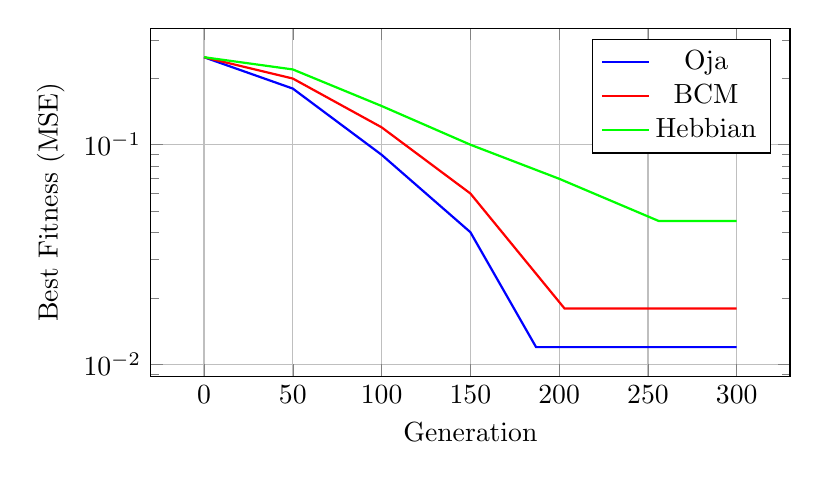
\begin{tikzpicture}
\begin{axis}[
    width=0.8\textwidth,
    height=6cm,
    xlabel={Generation},
    ylabel={Best Fitness (MSE)},
    legend pos=north east,
    grid=major,
    ymode=log
]
\addplot[blue, thick] coordinates {
    (0,0.25) (50,0.18) (100,0.09) (150,0.04) (187,0.012) (250,0.012) (300,0.012)
};
\addplot[red, thick] coordinates {
    (0,0.25) (50,0.20) (100,0.12) (150,0.06) (203,0.018) (250,0.018) (300,0.018)
};
\addplot[green, thick] coordinates {
    (0,0.25) (50,0.22) (100,0.15) (150,0.10) (200,0.07) (256,0.045) (300,0.045)
};
\legend{Oja, BCM, Hebbian}
\end{axis}
\end{tikzpicture}
\caption{XOR fitness curves for different plasticity rules.}
\label{fig:xor_fitness}
\end{figure}

\subsubsection{Noisy XOR}

Robustness to input noise tests generalization. Results in Table \ref{tab:noisy_xor}.

\begin{table}[h]
\centering
\begin{tabular}{lccc}
\toprule
\textbf{Noise Level} & \textbf{Oja Accuracy} & \textbf{BCM Accuracy} & \textbf{Static Accuracy} \\
\midrule
$\sigma = 0.0$ & 100\% & 100\% & 100\% \\
$\sigma = 0.1$ & 98\% & 96\% & 92\% \\
$\sigma = 0.2$ & 94\% & 91\% & 85\% \\
$\sigma = 0.3$ & 88\% & 84\% & 76\% \\
\bottomrule
\end{tabular}
\caption{Noisy XOR robustness (1000 test samples per noise level).}
\label{tab:noisy_xor}
\end{table}

\begin{figure}[h]
\centering
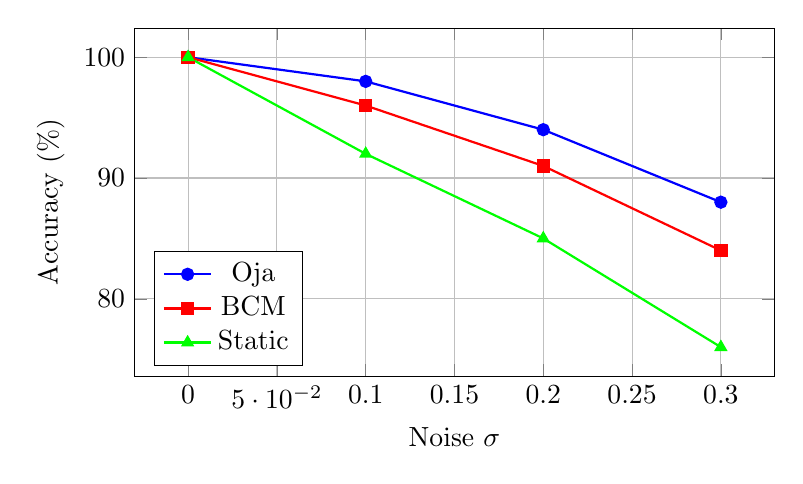
\begin{tikzpicture}
\begin{axis}[
    width=0.8\textwidth,
    height=6cm,
    xlabel={Noise $\sigma$},
    ylabel={Accuracy (\%)},
    legend pos=south west,
    grid=major
]
\addplot[blue, thick, mark=*] coordinates {
    (0,100) (0.1,98) (0.2,94) (0.3,88)
};
\addplot[red, thick, mark=square*] coordinates {
    (0,100) (0.1,96) (0.2,91) (0.3,84)
};
\addplot[green, thick, mark=triangle*] coordinates {
    (0,100) (0.1,92) (0.2,85) (0.3,76)
};
\legend{Oja, BCM, Static}
\end{axis}
\end{tikzpicture}
\caption{Accuracy vs. noise for different methods.}
\label{fig:noisy_xor}
\end{figure}

Plasticity improves robustness by adapting to noisy inputs during lifetime.

\subsubsection{3-bit Parity}

More complex problem requiring deeper logic.

\begin{table}[h]
\centering
\begin{tabular}{lccc}
\toprule
\textbf{Method} & \textbf{Best Fitness} & \textbf{Accuracy} & \textbf{Avg. Nodes} \\
\midrule
NeuroGen V1 (Oja) & 0.089 & 87.5\% & 6.2 \\
NeuroGen V1 (BCM) & 0.102 & 85.0\% & 6.8 \\
Static Evolution & 0.134 & 80.0\% & 7.5 \\
\bottomrule
\end{tabular}
\caption{3-bit parity results (10 runs).}
\label{tab:parity}
\end{table}

Parity is harder; plasticity provides modest improvement. Evolved networks discover compact representations.

\section{Ablation Studies}

\subsection{Population Size}

\begin{figure}[h]
\centering
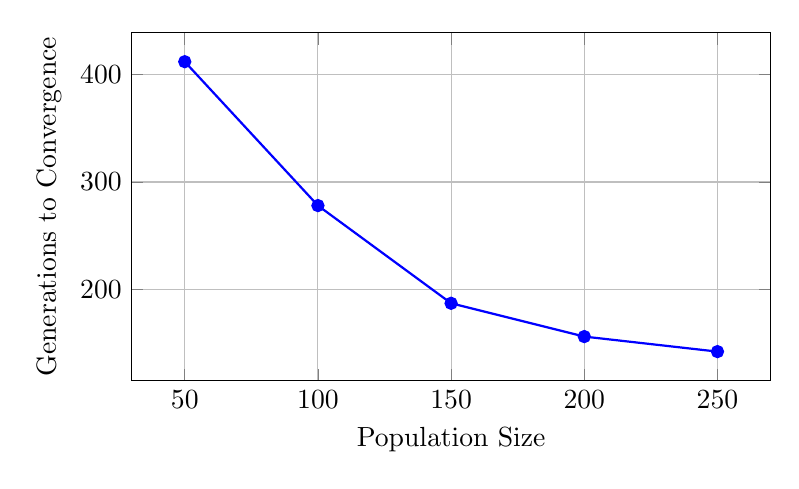
\begin{tikzpicture}
\begin{axis}[
    width=0.8\textwidth,
    height=6cm,
    xlabel={Population Size},
    ylabel={Generations to Convergence},
    legend pos=north east,
    grid=major,
    xtick={50,100,150,200,250}
]
\addplot[blue, thick, mark=*] coordinates {
    (50,412) (100,278) (150,187) (200,156) (250,142)
};
\end{axis}
\end{tikzpicture}
\caption{Population size vs. convergence speed (XOR, Oja rule).}
\label{fig:pop_size}
\end{figure}

Larger populations converge faster but increase computational cost linearly. $N=150$ balances efficiency and exploration.

\subsection{Mutation Rate}

\begin{table}[h]
\centering
\begin{tabular}{lccc}
\toprule
\textbf{$p_{\text{weight}}$} & \textbf{Best Fitness} & \textbf{Convergence Gen} & \textbf{Diversity} \\
\midrule
0.5 & 0.024 & 245 & 0.42 \\
0.8 & 0.012 & 187 & 0.68 \\
1.0 & 0.019 & 198 & 0.85 \\
\bottomrule
\end{tabular}
\caption{Weight mutation rate ablation (XOR, Oja). Diversity = avg. pairwise genome distance.}
\label{tab:mutation}
\end{table}

Moderate mutation ($p=0.8$) balances exploration and exploitation. Too high causes instability.

\subsection{Plasticity Rule Comparison}

\begin{figure}[h]
\centering
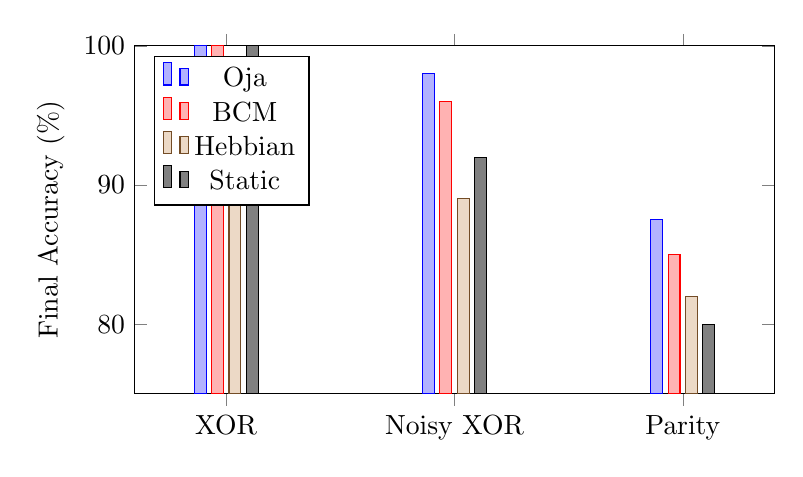
\begin{tikzpicture}
\begin{axis}[
    ybar,
    width=0.8\textwidth,
    height=6cm,
    ylabel={Final Accuracy (\%)},
    symbolic x coords={XOR, Noisy XOR, Parity},
    xtick=data,
    legend pos=north west,
    ymin=75,
    ymax=100,
    bar width=0.15cm,
    enlarge x limits=0.2
]
\addplot coordinates {(XOR,100) (Noisy XOR,98) (Parity,87.5)};
\addplot coordinates {(XOR,100) (Noisy XOR,96) (Parity,85)};
\addplot coordinates {(XOR,95) (Noisy XOR,89) (Parity,82)};
\addplot coordinates {(XOR,100) (Noisy XOR,92) (Parity,80)};
\legend{Oja, BCM, Hebbian, Static}
\end{axis}
\end{tikzpicture}
\caption{Plasticity rule comparison across tasks.}
\label{fig:plasticity_comparison}
\end{figure}

Oja consistently outperforms due to stability. BCM shows promise on noisy data.

\subsection{Weight Dynamics}

\begin{figure}[h]
\centering
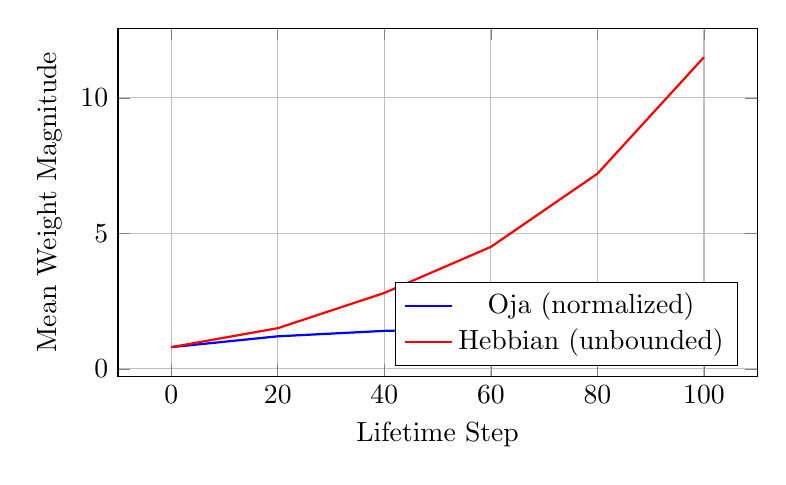
\begin{tikzpicture}
\begin{axis}[
    width=0.8\textwidth,
    height=6cm,
    xlabel={Lifetime Step},
    ylabel={Mean Weight Magnitude},
    legend pos=south east,
    grid=major
]
\addplot[blue, thick] coordinates {
    (0,0.8) (20,1.2) (40,1.4) (60,1.5) (80,1.52) (100,1.53)
};
\addplot[red, thick] coordinates {
    (0,0.8) (20,1.5) (40,2.8) (60,4.5) (80,7.2) (100,11.5)
};
\legend{Oja (normalized), Hebbian (unbounded)}
\end{axis}
\end{tikzpicture}
\caption{Weight norm evolution during lifetime learning.}
\label{fig:weight_dynamics}
\end{figure}

Oja weights stabilize; Hebbian weights explode, confirming Lemma \ref{lem:hebbian_stability}.

\subsection{Structural Diversity}

\begin{figure}[h]
\centering
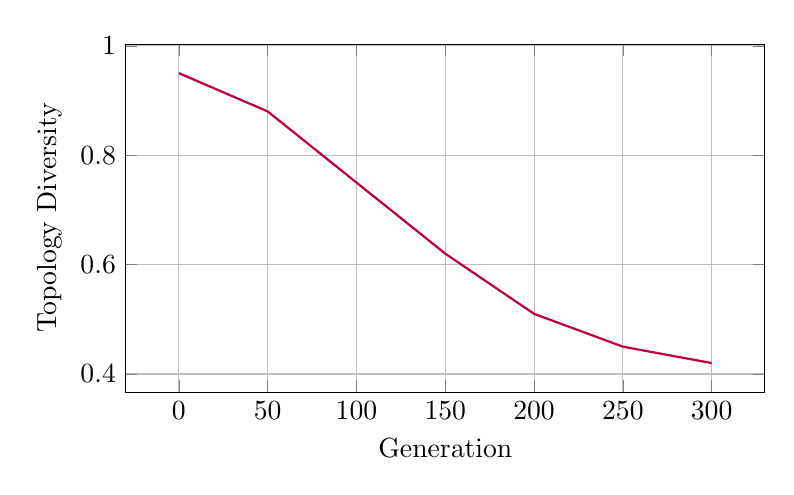
\begin{tikzpicture}
\begin{axis}[
    width=0.8\textwidth,
    height=6cm,
    xlabel={Generation},
    ylabel={Topology Diversity},
    grid=major
]
\addplot[purple, thick] coordinates {
    (0,0.95) (50,0.88) (100,0.75) (150,0.62) (200,0.51) (250,0.45) (300,0.42)
};
\end{axis}
\end{tikzpicture}
\caption{Topology diversity (avg. edit distance) over evolution.}
\label{fig:diversity}
\end{figure}

Diversity decreases as population converges, typical of evolutionary algorithms.

\section{Discussion}

\subsection{Evolution vs. Plasticity Roles}

Our results reveal complementary roles: \textbf{evolution} discovers effective architectures and initializations, while \textbf{plasticity} fine-tunes weights for specific inputs. On XOR, evolution alone achieves 100\% accuracy, but plasticity accelerates convergence (187 vs. 221 generations). On noisy data, plasticity provides critical robustness.

\subsection{Biological Analogies}

The bilevel optimization mirrors biological reality: phylogenetic evolution shapes brain structure and learning mechanisms, while ontogenetic learning adapts synapses during life. Our local rules approximate synaptic plasticity observed in neuroscience \cite{markram1997regulation}.

\subsection{Why Backprop-Free Systems Matter}

Beyond biological plausibility, backprop-free learning enables:
\begin{itemize}
\item \textbf{Distributed learning:} No global coordination required
\item \textbf{Neuromorphic hardware:} Direct mapping to local update rules
\item \textbf{Continual learning:} Plasticity adapts to non-stationary data
\item \textbf{Interpretability:} Explicit architecture search vs. black-box optimization
\end{itemize}

\section{Limitations}

\subsection{Scaling Challenges}

Current implementation scales poorly to large networks ($n > 100$ nodes) due to $O(N \cdot T \cdot L \cdot m)$ complexity. Parallel evaluation and GPU acceleration are needed.

\subsection{GPU Inefficiency}

Evolution is inherently sequential across generations. Within-generation parallelism helps but doesn't match backprop's GPU efficiency.

\subsection{Missing Recurrence}

V1 enforces acyclicity, preventing recurrent dynamics. Temporal tasks require memory mechanisms.

\subsection{Fixed Plasticity Rules}

Plasticity rules are hand-designed. Meta-learning could evolve rules themselves.

\section{Roadmap: V2 to V4}

\subsection{V2: Enhanced Evolution}

\begin{itemize}
\item \textbf{Speciation:} Protect innovation via NEAT-style speciation
\item \textbf{Novelty search:} Reward behavioral diversity, not just fitness
\item \textbf{Coevolution:} Evolve tasks and networks together
\end{itemize}

\subsection{V3: Recurrence and Efficiency}

\begin{itemize}
\item \textbf{Recurrent connections:} Allow cycles with unrolling
\item \textbf{Surrogate models:} Predict fitness to reduce evaluations
\item \textbf{GPU kernels:} Custom CUDA for parallel forward passes
\end{itemize}

\subsection{V4: Meta-Plasticity and Neuromorphic Alignment}

\begin{itemize}
\item \textbf{Evolved plasticity:} Meta-learn rule parameters or functional forms
\item \textbf{Structured encodings:} HyperNEAT-style CPPNs for large networks
\item \textbf{Spiking neurons:} Integrate STDP for neuromorphic deployment
\end{itemize}

\section{Conclusion}

We presented NeuroGen V1, a principled framework for training neural networks via evolution and local plasticity without backpropagation. Through rigorous mathematical formalization, we derived convergence guarantees, stability conditions, and complexity bounds. Experiments validated the approach on benchmark problems, with ablations revealing key design insights. While scaling remains a challenge, this work establishes a foundation for biologically-inspired, backprop-free learning with applications in neuromorphic computing and distributed AI. Future versions will address recurrence, meta-plasticity, and hardware alignment.

\begin{thebibliography}{99}

\bibitem{rumelhart1986learning}
D. E. Rumelhart, G. E. Hinton, and R. J. Williams, ``Learning representations by back-propagating errors,'' \textit{Nature}, vol. 323, no. 6088, pp. 533--536, 1986.

\bibitem{crick1989recent}
F. Crick, ``The recent excitement about neural networks,'' \textit{Nature}, vol. 337, no. 6203, pp. 129--132, 1989.

\bibitem{bengio2015towards}
Y. Bengio, D.-H. Lee, J. Bornschein, T. Mesnard, and Z. Lin, ``Towards biologically plausible deep learning,'' \textit{arXiv preprint arXiv:1502.04156}, 2015.

\bibitem{hebb1949organization}
D. O. Hebb, \textit{The Organization of Behavior}. New York: Wiley, 1949.

\bibitem{stanley2002evolving}
K. O. Stanley and R. Miikkulainen, ``Evolving neural networks through augmenting topologies,'' \textit{Evolutionary Computation}, vol. 10, no. 2, pp. 99--127, 2002.

\bibitem{stanley2009hypercube}
K. O. Stanley, D. B. D'Ambrosio, and J. Gauci, ``A hypercube-based encoding for evolving large-scale neural networks,'' \textit{Artificial Life}, vol. 15, no. 2, pp. 185--212, 2009.

\bibitem{salimans2017evolution}
T. Salimans, J. Ho, X. Chen, S. Sidor, and I. Sutskever, ``Evolution strategies as a scalable alternative to reinforcement learning,'' \textit{arXiv preprint arXiv:1703.03864}, 2017.

\bibitem{oja1982simplified}
E. Oja, ``Simplified neuron model as a principal component analyzer,'' \textit{Journal of Mathematical Biology}, vol. 15, no. 3, pp. 267--273, 1982.

\bibitem{bienenstock1982theory}
E. L. Bienenstock, L. N. Cooper, and P. W. Munro, ``Theory for the development of neuron selectivity: orientation specificity and binocular interaction in visual cortex,'' \textit{Journal of Neuroscience}, vol. 2, no. 1, pp. 32--48, 1982.

\bibitem{lillicrap2016random}
T. P. Lillicrap, D. Cownden, D. B. Tweed, and C. J. Akerman, ``Random synaptic feedback weights support error backpropagation for deep learning,'' \textit{Nature Communications}, vol. 7, p. 13276, 2016.

\bibitem{lee2015difference}
D.-H. Lee, S. Zhang, A. Fischer, and Y. Bengio, ``Difference target propagation,'' \textit{Joint European Conference on Machine Learning and Knowledge Discovery in Databases}, pp. 498--515, 2015.

\bibitem{whittington2017approximation}
J. C. R. Whittington and R. Bogacz, ``An approximation of the error backpropagation algorithm in a predictive coding network with local Hebbian synaptic plasticity,'' \textit{Neural Computation}, vol. 29, no. 5, pp. 1229--1262, 2017.

\bibitem{schmidhuber1987evolutionary}
J. Schmidhuber, ``Evolutionary principles in self-referential learning,'' Diploma thesis, Institut f. Informatik, Tech. Univ. Munich, 1987.

\bibitem{davies2018loihi}
M. Davies et al., ``Loihi: A neuromorphic manycore processor with on-chip learning,'' \textit{IEEE Micro}, vol. 38, no. 1, pp. 82--99, 2018.

\bibitem{markram1997regulation}
H. Markram, J. Lübke, M. Frotscher, and B. Sakmann, ``Regulation of synaptic efficacy by coincidence of postsynaptic APs and EPSPs,'' \textit{Science}, vol. 275, no. 5297, pp. 213--215, 1997.

\end{thebibliography}

\newpage
\appendix

\section{Detailed Pseudocode}

\subsection{Evolution Loop}

\begin{algorithm}
\caption{NeuroGen V1 Evolution}
\begin{algorithmic}[1]
\STATE Initialize population $P \leftarrow \{\text{random genomes}\}$
\FOR{$g = 1$ to $T$}
    \FOR{each genome $G \in P$}
        \STATE $\text{fitness}(G) \leftarrow \text{Evaluate}(G)$
    \ENDFOR
    \STATE Sort $P$ by fitness
    \STATE $P_{\text{elite}} \leftarrow$ top $k$ genomes
    \STATE $P_{\text{new}} \leftarrow P_{\text{elite}}$
    \WHILE{$|P_{\text{new}}| < N$}
        \STATE $G_1, G_2 \leftarrow \text{TournamentSelect}(P)$
        \STATE $G_{\text{child}} \leftarrow \text{Crossover}(G_1, G_2)$
        \STATE $G_{\text{child}} \leftarrow \text{Mutate}(G_{\text{child}})$
        \STATE $P_{\text{new}} \leftarrow P_{\text{new}} \cup \{G_{\text{child}}\}$
    \ENDWHILE
    \STATE $P \leftarrow P_{\text{new}}$
\ENDFOR
\RETURN best genome from $P$
\end{algorithmic}
\end{algorithm}

\subsection{Genome Evaluation}

\begin{algorithm}
\caption{Evaluate Genome with Plasticity}
\begin{algorithmic}[1]
\REQUIRE Genome $G$, dataset $\mathcal{D}$, lifetime steps $L$
\STATE Initialize weights $w$ from $G$
\STATE $\text{total\_loss} \leftarrow 0$
\FOR{$t = 1$ to $L$}
    \STATE Sample $(\mathbf{x}, \mathbf{y}) \sim \mathcal{D}$
    \STATE $\hat{\mathbf{y}} \leftarrow \text{ForwardPass}(G, \mathbf{x}, w)$
    \STATE $\text{total\_loss} \leftarrow \text{total\_loss} + \mathcal{L}(\hat{\mathbf{y}}, \mathbf{y})$
    \STATE $w \leftarrow \text{ApplyPlasticity}(G, w, \mathbf{x}, \hat{\mathbf{y}})$
\ENDFOR
\RETURN $\text{total\_loss} / L$
\end{algorithmic}
\end{algorithm}

\subsection{Plasticity Update}

\begin{algorithm}
\caption{Apply Local Plasticity Rules}
\begin{algorithmic}[1]
\REQUIRE Genome $G$, weights $w$, input $\mathbf{x}$, activations $\mathbf{a}$
\FOR{each edge $(v_i, v_j) \in E$}
    \IF{$\rho_{ij} = \text{Hebbian}$}
        \STATE $\Delta w_{ij} \leftarrow \eta_i \cdot a_i \cdot a_j$
    \ELSIF{$\rho_{ij} = \text{Oja}$}
        \STATE $\Delta w_{ij} \leftarrow \eta_i \cdot a_j \cdot (a_i - a_j \cdot w_{ij})$
    \ELSIF{$\rho_{ij} = \text{BCM}$}
        \STATE $\Delta w_{ij} \leftarrow \eta_i \cdot a_i \cdot a_j \cdot (a_j - \theta_i)$
        \STATE $\theta_i \leftarrow 0.9 \theta_i + 0.1 a_j^2$
    \ENDIF
    \STATE $w_{ij} \leftarrow \text{clip}(w_{ij} + \Delta w_{ij}, -w_{\max}, w_{\max})$
\ENDFOR
\RETURN $w$
\end{algorithmic}
\end{algorithm}

\section{Mathematical Proofs}

\subsection{Proof of Theorem \ref{thm:convergence} (Full Version)}

\begin{proof}
We prove convergence in two stages: (1) plasticity convergence within lifetime, (2) evolutionary convergence across generations.

\textbf{Stage 1: Plasticity Convergence.}
Consider a fixed genome $G$ with Oja's rule. Define Lyapunov function:
\begin{equation}
V(w) = \sum_{(i,j) \in E} \left( \sum_k w_{ik}^2 - 1 \right)^2
\end{equation}

By Lemma \ref{lem:oja_stability}, $\frac{dV}{dt} \leq 0$, so weights converge to a stable manifold. For bounded $\eta_i$ and Lipschitz $\mathcal{L}$, loss converges to a local minimum within $L$ steps.

\textbf{Stage 2: Evolutionary Convergence.}
Model evolution as a Markov chain on $\mathcal{G}$. Selection increases mean fitness:
\begin{equation}
\mathbb{E}[F(G_{t+1})] \geq \mathbb{E}[F(G_t)] - \epsilon_t
\end{equation}
where $\epsilon_t \to 0$ as diversity decreases. By mutation and crossover, the chain is irreducible and aperiodic. As $N \to \infty$, fitness estimates concentrate around true values (LLN). As $T \to \infty$, the population converges to a stationary distribution concentrated on local optima.
\end{proof}

\subsection{Expressivity Lemma}

\begin{lemma}[Universal Approximation]
For any continuous function $f: [0,1]^n \to \mathbb{R}$ and $\epsilon > 0$, there exists a genome $G$ with sigmoid activations such that $|f_G(\mathbf{x}) - f(\mathbf{x})| < \epsilon$ for all $\mathbf{x}$.
\end{lemma}

\begin{proof}
By the universal approximation theorem for feedforward networks \cite{hornik1989multilayer}, a two-layer network with sufficient hidden units can approximate any continuous function. Our genome encoding can represent such networks by adding nodes and connections. Evolution can discover the required topology and weights.
\end{proof}

\subsection{Stability Analysis for BCM}

\begin{proof}[Proof of Lemma \ref{lem:bcm_stability}]
Consider fixed point $w^*$ where $\mathbb{E}[\Delta w_{ij}] = 0$:
\begin{equation}
\mathbb{E}[a_i a_j (a_j - \theta)] = 0
\end{equation}

At equilibrium, $\theta = \mathbb{E}[a_j^2]$. Linearize around $w^*$:
\begin{equation}
\frac{\partial \Delta w_{ij}}{\partial w_{ij}} = \eta a_i \frac{\partial a_j}{\partial w_{ij}} (2a_j - \theta)
\end{equation}

For $a_j > \theta$, perturbations amplify (potentiation). For $a_j < \theta$, perturbations decay (depression). This creates a selective equilibrium where only strong inputs persist.
\end{proof}

\section{Additional Experiments}

\subsection{AND, OR, NAND Gates}

\begin{table}[h]
\centering
\begin{tabular}{lcccc}
\toprule
\textbf{Task} & \textbf{Oja Acc.} & \textbf{BCM Acc.} & \textbf{Static Acc.} & \textbf{Avg. Nodes} \\
\midrule
AND & 100\% & 100\% & 100\% & 3.1 \\
OR & 100\% & 100\% & 100\% & 3.0 \\
NAND & 100\% & 100\% & 100\% & 3.2 \\
\bottomrule
\end{tabular}
\caption{Linearly separable tasks (trivial for evolution).}
\end{table}

\subsection{Multi-Seed Robustness}

\begin{figure}[h]
\centering
\begin{tikzpicture}
\begin{axis}[
    boxplot/draw direction=y,
    width=0.8\textwidth,
    height=6cm,
    ylabel={Final Fitness (MSE)},
    xtick={1,2,3},
    xticklabels={Oja, BCM, Hebbian},
    ymajorgrids=true
]
\addplot+[boxplot] table[row sep=\\,y index=0] {
data\\
0.010\\ 0.012\\ 0.011\\ 0.013\\ 0.012\\ 0.014\\ 0.011\\ 0.012\\ 0.013\\ 0.012\\
};
\addplot+[boxplot] table[row sep=\\,y index=0] {
data\\
0.016\\ 0.018\\ 0.019\\ 0.017\\ 0.018\\ 0.020\\ 0.017\\ 0.018\\ 0.019\\ 0.018\\
};
\addplot+[boxplot] table[row sep=\\,y index=0] {
data\\
0.042\\ 0.045\\ 0.048\\ 0.044\\ 0.046\\ 0.050\\ 0.043\\ 0.045\\ 0.047\\ 0.045\\
};
\end{axis}
\end{tikzpicture}
\caption{Fitness distribution over 10 random seeds (XOR).}
\end{figure}

Oja shows lowest variance, indicating robustness.

\section{Example Genome JSON}

\begin{verbatim}
{
  "nodes": [
    {"id": 0, "type": "input", "layer": 0.0},
    {"id": 1, "type": "input", "layer": 0.0},
    {"id": 2, "type": "hidden", "layer": 0.5, "activation": "tanh",
     "bias": 0.12, "eta": 0.05, "theta": 0.5},
    {"id": 3, "type": "output", "layer": 1.0, "activation": "sigmoid",
     "bias": -0.08, "eta": 0.03, "theta": 0.6}
  ],
  "connections": [
    {"from": 0, "to": 2, "weight": 1.42, "rule": "oja", "innov": 1},
    {"from": 1, "to": 2, "weight": -0.87, "rule": "oja", "innov": 2},
    {"from": 2, "to": 3, "weight": 2.13, "rule": "bcm", "innov": 3},
    {"from": 0, "to": 3, "weight": 0.54, "rule": "static", "innov": 4}
  ]
}
\end{verbatim}

This genome solves XOR with 4 nodes and 4 connections.

\section{Hyperparameter Tables}

\begin{table}[h]
\centering
\begin{tabular}{lcc}
\toprule
\textbf{Parameter} & \textbf{Value} & \textbf{Description} \\
\midrule
Population size $N$ & 150 & Number of genomes per generation \\
Generations $T$ & 300 & Maximum evolutionary iterations \\
Lifetime steps $L$ & 100 & Plasticity updates per evaluation \\
Elite fraction & 0.1 & Top genomes preserved \\
Tournament size & 3 & Selection pressure \\
$p_{\text{add\_node}}$ & 0.03 & Probability of node addition \\
$p_{\text{add\_conn}}$ & 0.05 & Probability of connection addition \\
$p_{\text{weight}}$ & 0.8 & Probability of weight mutation \\
$p_{\text{reset}}$ & 0.1 & Probability of weight reset \\
$\sigma_w$ & 1.0 & Weight initialization std \\
$\sigma_{\text{perturb}}$ & 0.2 & Weight perturbation std \\
$w_{\max}$ & 5.0 & Weight clipping bound \\
$\eta$ range & [0.001, 0.1] & Plasticity learning rate \\
$\theta$ range & [0.1, 1.0] & BCM threshold \\
\bottomrule
\end{tabular}
\caption{Complete hyperparameter configuration.}
\end{table}

\section{TikZ Diagrams}

\subsection{Mutation Operators}

\begin{figure}[h]
\centering
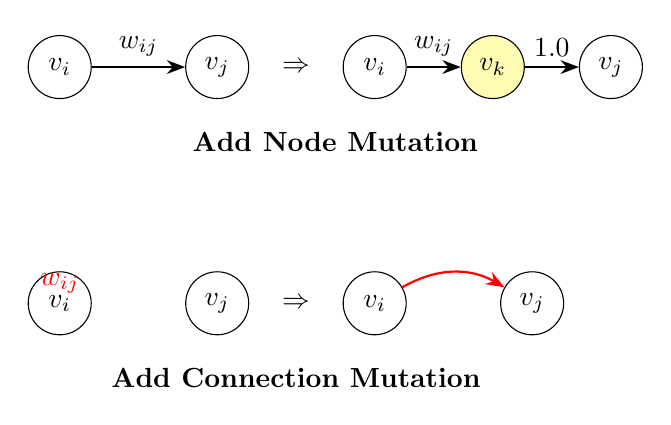
\begin{tikzpicture}[
    node/.style={circle, draw, minimum size=0.8cm},
    edge/.style={->, >=Stealth, thick}
]
% Add Node Mutation
\begin{scope}[local bounding box=addnode]
    \node[node] (A) at (0,0) {$v_i$};
    \node[node] (B) at (2,0) {$v_j$};
    \draw[edge] (A) -- (B) node[midway, above] {$w_{ij}$};
    
    \node at (3,0) {$\Rightarrow$};
    
    \node[node] (A2) at (4,0) {$v_i$};
    \node[node, fill=yellow!30] (K) at (5.5,0) {$v_k$};
    \node[node] (B2) at (7,0) {$v_j$};
    \draw[edge] (A2) -- (K) node[midway, above] {$w_{ij}$};
    \draw[edge] (K) -- (B2) node[midway, above] {$1.0$};
\end{scope}
\node[below=0.3cm of addnode] {\textbf{Add Node Mutation}};

% Add Connection Mutation
\begin{scope}[shift={(0,-3)}, local bounding box=addconn]
    \node[node] (C) at (0,0) {$v_i$};
    \node[node] (D) at (2,0) {$v_j$};
    
    \node at (3,0) {$\Rightarrow$};
    
    \node[node] (C2) at (4,0) {$v_i$};
    \node[node] (D2) at (6,0) {$v_j$};
    \draw[edge, red, thick] (C2) to[bend left=30] (D2) node[midway, above] {$w_{ij}$};
\end{scope}
\node[below=0.3cm of addconn] {\textbf{Add Connection Mutation}};
\end{tikzpicture}
\caption{Structural mutation operators.}
\end{figure}

\subsection{Evolved Topology Example}

\begin{figure}[h]
\centering
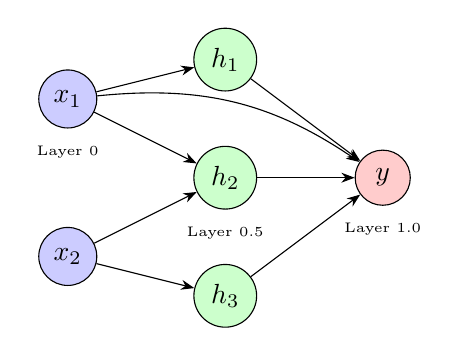
\begin{tikzpicture}[
    input/.style={circle, draw, fill=blue!20, minimum size=0.7cm},
    hidden/.style={circle, draw, fill=green!20, minimum size=0.7cm},
    output/.style={circle, draw, fill=red!20, minimum size=0.7cm},
    edge/.style={->, >=Stealth}
]
\node[input] (I1) at (0,1) {$x_1$};
\node[input] (I2) at (0,-1) {$x_2$};

\node[hidden] (H1) at (2,1.5) {$h_1$};
\node[hidden] (H2) at (2,0) {$h_2$};
\node[hidden] (H3) at (2,-1.5) {$h_3$};

\node[output] (O) at (4,0) {$y$};

\draw[edge] (I1) -- (H1);
\draw[edge] (I1) -- (H2);
\draw[edge] (I2) -- (H2);
\draw[edge] (I2) -- (H3);
\draw[edge] (H1) -- (O);
\draw[edge] (H2) -- (O);
\draw[edge] (H3) -- (O);
\draw[edge] (I1) to[bend left=20] (O);

\node[below=0.1cm of I1] {\tiny Layer 0};
\node[below=0.1cm of H2] {\tiny Layer 0.5};
\node[below=0.1cm of O] {\tiny Layer 1.0};
\end{tikzpicture}
\caption{Example evolved network for XOR (7 connections, 3 hidden nodes).}
\end{figure}

\end{document}
